%%%%% Please set the path to 'beamer' directory in your environment %%%%%
\newcommand{\beamerDir}[0]{/mnt/c/Users/atsushi/Documents/workspace/env/Beamer/beamer/beamer/}


%%%%% Load setting %%%%%
\documentclass[aspectratio=169, dvipdfmx, 12pt, compress]{beamer}% dvipdfmxしたい

%%%%% Packages %%%%%
\usepackage{bxdpx-beamer}% dvipdfmxなので必要
\usepackage{pxjahyper}% 日本語で'しおり'したい
\usepackage{tikz}
\usepackage{tcolorbox}
\usetikzlibrary{shapes}
\usepackage{xcolor}
\usepackage[absolute,overlay]{textpos}
\usepackage{adjustbox}
\usepackage{caption}
\usepackage{ifthen}


%%%%% Settings %%%%%
\usetheme[sectionpage=progressbar, subsectionpage=progressbar]{metropolis}
% block style
\metroset{block=fill}
% space between line
\renewcommand{\baselinestretch}{1.3}
% space between item
\newlength{\wideitemsep}
\setlength{\wideitemsep}{0.9\itemsep}
% \addtolength{\wideitemsep}{1.0pt} <- more space
\let\olditem\item
\renewcommand{\item}{\setlength{\itemsep}{\wideitemsep}\olditem}
% frame title
\definecolor{coolblack}{rgb}{0.0, 0.18, 0.39}
\setbeamercolor{frametitle}{bg=coolblack!90,fg=white}
\setbeamerfont{frametitle}{size=\large}
\addtobeamertemplate{frametitle}{}{\vspace{-1em}}
\makeatletter
\setlength{\metropolis@frametitle@padding}{1.4ex}% <- default 2.2 ex
% foot line
\addtobeamertemplate{footline}{}{\vspace{-1em}}
% normal text color
\setbeamercolor{normal text}{fg=black!80}
% progress bar
\definecolor{lightgray}{rgb}{0.83, 0.83, 0.83}
\setbeamercolor{progress bar}{bg=lightgray, fg=coolblack}
\setbeamersize{text margin left=15pt, text margin right=15pt}
% equation font
\usefonttheme{professionalfonts}
% Change standard block width
\addtobeamertemplate{block begin}{%
    \centering
    \begin{columns}\begin{column}{0.9\textwidth}
            \centering
            }{}
            \addtobeamertemplate{block end}{}{\end{column}\end{columns}}
% Change alert block width
\addtobeamertemplate{block alerted begin}{%
    \centering
    \begin{columns}\begin{column}{0.9\textwidth}
            \centering
            }{}
            \addtobeamertemplate{block alerted end}{}{\end{column}\end{columns}}
% Change example block width
\addtobeamertemplate{block example begin}{%
    \centering
    \begin{columns}\begin{column}{0.9\textwidth}
            \centering
            }{}
            \addtobeamertemplate{block example end}{}{\end{column}\end{columns}}
% Itemize color
\setbeamertemplate{itemize item}{\color{black}\scriptsize$\blacksquare$}
\setbeamertemplate{itemize subitem}{\color{black}\scriptsize$-$}
% Simplification  color
\definecolor{cobalt}{rgb}{0.0, 0.28, 0.67}
\setbeamercolor{block title example}{fg=black!80,bg=cobalt!35}
\setbeamercolor{block body example}{fg=black,bg=cobalt!15}
% Definition
\BeforeBeginEnvironment{definition}{
    \setbeamercolor{block title}{use=alerted text, bg=alerted text.fg!70,fg=white}
    \setbeamercolor{block body}{use=alerted text, bg=alerted text.fg!20}
}
\AfterEndEnvironment{definition}{% return to default
    \setbeamercolor{block title}{use=structure,fg=structure.fg,bg=structure.fg!20!bg}
    \setbeamercolor{block body}{parent=normal text,use=block title,bg=block title.bg!50!bg, fg=black}
}
% Theorem
\definecolor{seagreen}{rgb}{0.18, 0.55, 0.34}
\setbeamertemplate{theorems}[numbered]
\BeforeBeginEnvironment{theorem}{
    \setbeamercolor{block title}{fg=black!80,bg=seagreen!40}
    \setbeamercolor{block body}{fg=black,bg=seagreen!15}
}
\AfterEndEnvironment{theorem}{% return to default
    \setbeamercolor{block title}{use=structure,fg=structure.fg,bg=structure.fg!20!bg}
    \setbeamercolor{block body}{parent=normal text,use=block title,bg=block title.bg!50!bg, fg=black}
}
% Lemma
\undef{\lemma}
\newtheorem{lemma}{\translate{Lemma}}
\BeforeBeginEnvironment{lemma}{
    \setbeamercolor{block title}{fg=black!80,bg=seagreen!20}
    \setbeamercolor{block body}{fg=black,bg=seagreen!10}
}
\AfterEndEnvironment{lemma}{% return to default
    \setbeamercolor{block title}{use=structure,fg=structure.fg!80,bg=structure.fg!20!bg}
    \setbeamercolor{block body}{parent=normal text,use=block title,bg=block title.bg!50!bg, fg=black}
}


%%%%% Original Command %%%%%
\newcommand{\subt}[1]{\vspace{-2mm}{\fontsize{10pt}{0cm}\selectfont \textcolor{lightgray}{#1}}\vspace{-1mm}}
\newcommand{\lastpage}[0]{\begin{frame}\begin{textblock*}{1.0\linewidth}(0pt, 50pt)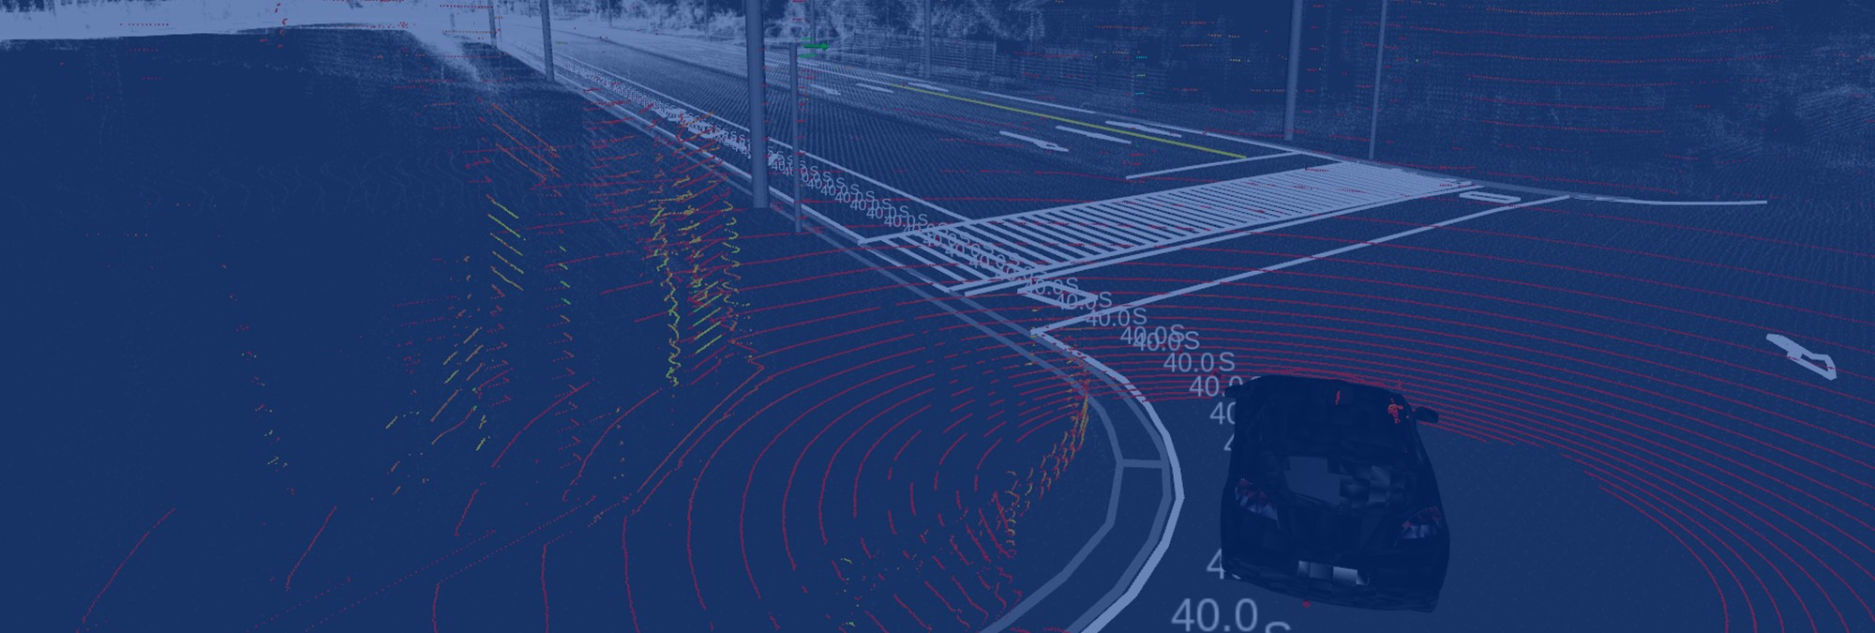
\includegraphics[scale=0.512]{\beamerDir/master_figure/last.pdf}\end{textblock*}\end{frame}}
\newcommand{\todo}[1]{\al{\LARGE\textbf{TODO:} #1}}
\newcommand{\headerheight}[0]{5mm}
\newcommand{\footerheight}[0]{5mm}
\newcommand{\slideheight}[0]{\textheight-\headerheight-\footerheight}
\newcommand{\tabml}[1]{\hspace{-2.1mm}\begin{tabular}{l} #1 \end{tabular}}
\newcommand{\al}[1]{\alert{#1}}
\newcommand{\argempty}[0]{}
\newcommand{\onlyslide}[1]{
    \vspace{\headerheight}
    \begin{minipage}[c][\slideheight][c]{\textwidth}
        #1
    \end{minipage}
}
\newcommand{\onlyimage}[1]{
    \onlyslide{
        \centering
        \begin{columns}
            \begin{column}{\textwidth}
                \centering
                \adjustbox{max width=\textwidth, max height=\slideheight}{
                    \includegraphics{#1}
                }
            \end{column}
        \end{columns}
    }
}
% fit image
\newlength\fitimageht
\newlength\fitotherht
\newsavebox\fitimagebox
\newcommand{\fitimage}[2]{%
    \sbox\fitimagebox{%
        \parbox{\textwidth}{%
            #1\par
        }%
    }%
    \settototalheight{\fitotherht}{%
        \usebox\fitimagebox
    }%
    \setlength\fitimageht{\textheight}%
    \addtolength\fitimageht{-\fitotherht-\headerheight-\footerheight-1\baselineskip}%
    \vspace{\headerheight}
    #1\par
    \centering
    \includegraphics[width=\textwidth,height=\fitimageht,keepaspectratio]{#2}
}
% Simplification
\newcommand{\assume}[1]{
    \begin{exampleblock}{Simplification }
        #1
    \end{exampleblock}
}
% Re-post
\setbeamercolor{RepostBox}{fg=black!50, bg=coolblack!10}
\newcommand{\repost}[1]{
    \vspace{2mm}
    \centering
    \begin{columns}
        \begin{column}{0.86\textwidth}
            \begin{beamercolorbox}[wd=\textwidth, sep=2pt, rounded=true, shadow=true]{RepostBox}
                \begin{tabular}{|p{0.95\textwidth}}
                    {\fontsize{10pt}{10pt}#1}
                \end{tabular}
            \end{beamercolorbox}
        \end{column}
    \end{columns}
}

% equation ballon
\tcbset{
    framebox/.style={
            enhanced,
            boxsep=0pt,       % 箱の上下左右の余白を指定
            colback=white,
            boxrule=1pt,
            colframe=#1
        },
    framebox/.default=red
}
\newcommand{\upbln}[3]{
    \tcboxmath[
        framebox=#2,
        top=0.5ex,bottom=0.5ex,    % 箱の上下の余白を指定
        left=0.5ex,right=0.5ex,    % 箱の左右の余白を指定
        overlay={
                \node[
                    above,
                    rectangle callout,                         % nodeを吹き出しの形に
                    callout absolute pointer={(frame.north)},  % 吹き出しの先端を絶対的に指定
                    fill=#2!20
                ] at ([yshift=2ex]frame.north) {\footnotesize#3};
            }
    ]{#1}
}
\newcommand{\lwbln}[3]{
    \tcboxmath[
        framebox=#2,
        top=0.5ex,bottom=0.5ex,    % 箱の上下の余白を指定
        left=0.5ex,right=0.5ex,    % 箱の左右の余白を指定
        overlay={
                \node[
                    below,
                    rectangle callout,                         % nodeを吹き出しの形に
                    callout absolute pointer={(frame.south)},  % 吹き出しの先端を絶対的に指定
                    fill=#2!20
                ] at ([yshift=-2ex]frame.south) {\footnotesize#3};
            }
    ]{#1}
}
\tcbuselibrary{theorems,skins}



%%%%% Mode %%%%%
% \newcommand{\forme}[1]{#1}
\newcommand{\forme}[1]{}


%%%%% Front Cover %%%%%
\title{Analysis of Federated and Global Scheduling for Parallel Real-Time Tasks}
\subtitle{IEEE Real-Time Systems Symposium (RTSS), 2014}
\author{矢野 篤志}
\date{\today}
\institute[EMBIV]{EMBIV}
\logo{\begin{textblock*}{0.1\linewidth}(2pt, 237pt)
\includegraphics[scale=0.4]{\beamerDir/master_figure/Emb_logo.pdf}\end{textblock*}}


%%%%% Document Start %%%%%
\begin{document}

\maketitle

\summary{2}{0}
% !TeX root = main.tex


\begin{frame}{提案の概要}
    \begin{itemize}
        \item 優先度駆動型スケジューリングによってROSのリアルタイム性能と予測可能性を大幅に改善できることを主張する
        \item 主張を裏付けるために, 優先度駆動型チェーン考慮スケジューリングに関する我々の研究をレビューし, Apex.AI が開発したオープンソースリファレンスシステムを用いた評価を行う
        \item ROS 2のリアルタイム性能を向上させるために不可欠な以下2つの課題を説明する
        \begin{itemize}
            \item マルチスレッドエグゼキュータ設計
            \item アクセラレータサポート
        \end{itemize}
    \end{itemize}
\end{frame}


\begin{frame}{Outline}
    \setbeamertemplate{section in toc}[sections numbered]
    \scriptsize\tableofcontents[hideallsubsections]
\end{frame}

% !TeX root = main.tex

\section{PRIOR KNOWLEDGE}
\label{sec: prior knowledge}

\begin{frame}{前提知識}
    \begin{itemize}
        \item \ourl{ROS}{https://tier4.atlassian.net/wiki/spaces/EMBIV/pages/2683603071/ROS+Robot+Operating+System}
        \item \ourl{publish/subscribeモデル}{https://tier4.atlassian.net/wiki/spaces/EMBIV/pages/2675048610/Publish+Subscribe}
        \item \ourl{SCHED\_DEADLINE}{https://tier4.atlassian.net/wiki/spaces/EMBIV/pages/2692645566/SCHED+DEADLINE}
        \item \ourl{最大イベント到着曲線}{https://drive.google.com/file/d/1n85X0vDrDm4IDANDP4aUoC0SNnZLAiRN/view?usp=share_link}
        \item \ourl{Casiniらによる先行研究}{https://drive.google.com/file/d/1sHujFqbmgCoJbC6g6KdC7ihua4Jqddju/view?usp=share_link}
    \end{itemize}
\end{frame}

% !TeX root = main.tex

\section{INTRODUCTION}
\label{sec: introduction}

\begin{frame}{}
    \begin{itemize}
        \item ロボット工学のような, 様々な分野の深い専門知識を必要とする学際的で複雑なアプリケーション領域では, 通常, 全ての, あるいはほとんどのソフトウェアをゼロから書くという選択肢はあり得ない
        \item その代わりに, ロボット工学者は, ROSのような一般的なロボット工学フレームワークで容易に利用できる, 標準機能を提供する既存のサードパーティコンポーネントの統合を採用するのが一般的である
        \item その利点は数多く, 簡単に理解できる
        \item 例えば, 複数の最新パス計画アルゴリズムと3D可視化サポートを備えた完全なナビゲーションスタックがたった1回のダウンロードで手に入るなら, なぜ新しいナビゲーションサブシステムを苦労して開発する必要があるか?
    \end{itemize}
\end{frame}

\begin{frame}{}
    \begin{itemize}
        \item 完全なロボットシステムを構築するためには, 多くの相互作用するコンポーネントを統合する必要がある
        \item ROS開発プロセスの分散型オープンソースの性質により, これらのコンポーネントは通常, 必ずしもお互いを知らない複数の独立したコンポーネント開発者によって分離して開発される
        \item 同様に, システムインテグレータは, アプリケーションおよびミッション固有のロジックと「グルーコード」で展開プラットフォーム上で選択したコンポーネントを構成するが, 通常, それぞれのコンポーネント開発者と密接に連携することはない
    \end{itemize}
\end{frame}

\begin{frame}{}
    \begin{itemize}
        \item コンポーネントの統合を可能な限りシンプルに保つために, ROSはコンポーネントの疎結合を可能にする古典的なトピックベースのpublish/subscribeパラダイムを採用している
        \item 概念的には, 各コンポーネントは, 特定のトピックをsubscribeする多数のコールバックを含む「ブラックボックス」として理解できる
        \item 与えられたトピックに関連するメッセージがpublishされるたびに, 全てのsubscribeコールバックが呼び出され, 何らかの計算を実行し, 次に他のトピックに後続のメッセージをpublishすることができ, これがさらにコールバックをトリガするというように, 繰り返す
    \end{itemize}
\end{frame}

\begin{frame}{}
    \begin{itemize}
        \item インテグレータは, あるコンポーネントの「入力コールバック」を別のコンポーネントの「出力トピック」に接続することによってコンポーネントを構成する
        \item ROSシステムは, このように相互接続されたトピックとコールバックの複雑なネットワークを形成し, データ (環境刺激など) は, イベント駆動型の方法でネットワークを通じてcause-effectチェーンに沿って伝播し, インテグレータが望むように透過的にコンポーネント境界を交差させることができる
    \end{itemize}
\end{frame}

\begin{frame}{}
    \begin{itemize}
        \item このようなcause-effectチェーンの典型的な例として, 進路上の障害物を検知して反応する必要のある移動ロボットのセンシング-計算-行動パイプラインが挙げられる
        \item 例えば, ハードウェアドライバコンポーネントがレーザースキャナから新しいサンプルを取得し (cause) , それが複数のマッピング, 座標変換, パス計画, 車輪制御コンポーネントを経て, 最終的に車輪速度の変化 (effect) をもたらす可能性がある
        \item このようなデータ処理のチェーンにおいて, causeからeffectまでの最大レイテンシ時間は, ロボットが正しく機能するために重要な役割を果たすことは明らかであり, また, 安全性を考慮する上でも重要であることが多い
    \end{itemize}
\end{frame}

\begin{frame}{}
    \begin{itemize}
        \item 重要なのは, システムインテグレータにできるだけ多くの展開の選択肢を残し, コンポーネントの再利用の機会を最大化するために, ROSの実行管理層と基礎となるオペレーティングシステムは, 意図的にコンポーネント開発者に公開されないことである
        \item むしろ, ROSの中心的なコールバック抽象化は, コールバック手続きがいつどのようにスケジュールされるか, コールバックの実行がスレッドまたはプロセスにわたってどのように組織されるか, またはネットワーキング層がメッセージの送受信をどのように処理するかを全く意識せずに, 実行から完了までセマンティクスを持つ単なる手続きである
    \end{itemize}
\end{frame}

\begin{frame}{}
    \begin{itemize}
        \item ROSはオープンソースソフトウェアであるため, 原理的にはシステムの実行と通信の挙動を完全に理解し制御することが可能である
        \item このため, リアルタイムシステムの専門家から見れば, ROSにリアルタイムシステム研究でよく知られた技術を導入することは論理的なステップであるように思える可能性がある
        \item しかし, 一見したところ, これを難しくしているハードルがいくつかある
    \end{itemize}
\end{frame}

\begin{frame}{}
    \begin{itemize}
        \item まず第一に, インテグレータに必要な情報が不足している
        \item ほとんどのリアルタイム分析では, 同時実行タスクの数, それらの起動セマンティクスや機能的相互作用, メッセージの到着パターン, 最悪実行時間など, 多くの低レベルシステムの詳細に関する深い知識が前提となっている
        \item ROSコンポーネントは, この種の情報を提供するマニフェストと一緒に来ることはない
        \item さらに悪いことに, リアルタイム分析は, 欠陥のある情報や不完全な情報にうまく対処できない
        \item モデリング目的でサードパーティコンポーネントを手作業でリバースエンジニアリングしているときに, たった一つのミスや見落としがあれば, その取り組み全体を無条件に無効にしてしまうことになりかねない
    \end{itemize}
\end{frame}

\begin{frame}{}
    \begin{itemize}
        \item 第二に, 必要なシステムの詳細をコンポーネントレベルで静的に決定し, 記述することができない
        \item その理由のひとつは, 多くのロボット工学アルゴリズムが, ユースケースやプラットフォーム固有の側面に依存し, 実行時間や起動パターンが大きく変化するためである
        \item 例えば, ビデオストリーム中の物体を識別し, その軌跡を推測する一般的な物体追跡コンポーネントを考えてみよう (例えば, 隣の車線の車など)
        \item この機能の実行時間は, ビデオストリームのフレームレート, 解像度, コーデック, および特定のトラッキングアルゴリズムに関連する他の様々なパラメータを含む, 様々なパラメータに依存する
        \item これらのパラメータは, 一般的なオブジェクトトラッキングコンポーネントの開発者が前もって知っていたり, 固定されていたりするものではない
    \end{itemize}
\end{frame}

\begin{frame}{}
    \begin{itemize}
        \item このようなユースケース特有の情報は, 特定のロボットを構築するインテグレーターにしか分からない
        \item インテグレーターは, 必ずしもオブジェクトトラッキングやリアルタイムシステムの専門家ではないため, 特定の構成を選択した場合の影響を常に予測できるわけではない
        \item したがって, コンポーネントのリソース要求とリアルタイム動作は, 常に特定の展開で使用するという文脈で評価されなければならない
        \item これは, ROSフレームワークの人気の根底にある「ブラックボックス」コンポーネントのモジュール式再利用と相容れるものではない
    \end{itemize}
\end{frame}

\begin{frame}{}
    \begin{itemize}
        \item 最後に, 仮にインテグレータが各コンポーネントについてそれぞれの専門家と議論し, タイミング分析に必要な全ての詳細を入手できたとしても, 第三の根本的な問題が残る
        \item 多くのコンポーネントのリソース要件と性能特性は, 本質的にロボットの動的環境に依存し, したがって時間とともに変化するため, 静的 (最悪のケース) リソース配置は実行不可能なのである
    \end{itemize}
\end{frame}

\begin{frame}{}
    \begin{itemize}
        \item 例えば, 前述の物体追跡コンポーネントと, ランドマークベースの自己位置特定コンポーネントに依存するロボットを再度考えてみよう
        \item 一方, 人口が少ない田舎町よりも, にぎやかな街中を移動する方が, 物体追跡装置の処理時間はずっと長くなる
        \item 一方, 認識可能なランドマークが多い都市部では, ほぼ一様な風景よりも自己位置推定がはるかに容易である可能性が高い
        \item どちらの状況でも十分なリソースを確保するためには, システムインテグレーターは, 不毛の土地からなる賑やかな都市を想定したシステムを用意しなければならない
    \end{itemize}
\end{frame}

\begin{frame}{}
    \begin{itemize}
        \item ロボット工学では, このような悲観的なシステム設計を行うと, すぐに現実的な限界に直面することになる
        \item その代わりに, 実用的で費用対効果の高いシステムを維持するためには, 各コンポーネントのピーク需要の合計ではなく, 予想されるジョイントリソースのピーク需要に対してプロビジョニングを行う必要がある
    \end{itemize}
\end{frame}

\begin{frame}{貢献する}
    \begin{itemize}
        \item これらの課題を克服するために, 我々は, 実行時に動的にタイミングを考慮した方法でROSシステムをプロビジョニングするための自動レイテンシマネージャを使用することを提案する
        \item 具体的には, ROS Live latency manager (ROSLlama) を紹介する
        \item これは, 重要なcause-effectチェーンに沿ったレイテンシを, 非リアルタイム専門家が使いやすく, かつ設定にあまり手間をかけない方法で, 既存のリアルタイム機構を使用して制御することを可能にする
    \end{itemize}
\end{frame}

\begin{frame}{貢献する}
    \begin{itemize}
        \item ROS-Llamaは, 複雑なシステムパラメータをユーザに要求するのではなく, 実行時に必要なパラメータを自動的に推定し, 状況の変化に応じてスケジューリングパラメータを動的に調整することが可能である
        \item もし, 指定されたレイテンシの目標が全て同時に達成できない場合 (例えば, 不利な環境条件による一時的な過負荷が原因) , ROS-Llamaは制御された緩やかなデグレードプロセスを開始し, システムインテグレーターが純粋に宣言的な方法で (すなわち, cause-effectチェーンがどの部品を通過しているかを理解しなくても) cause-effectチェーンの重要性を特定できるようにする
    \end{itemize}
\end{frame}

\begin{frame}{本論文の貢献}
    \begin{itemize}
        \item  ロボティクス領域における動的レイテンシ管理問題を探求し, 実用的なソリューションが満たさなければならない制約と要件を文書化する (第III章)

        \item  ROSのための最初の自動レイテンシマネージャであるROS-Llamaの設計と実装を紹介する (セクションIV)

        \item 標準的な Linux システム上の ROS コンポーネントを用いて, ROS-Llama が移動ロボットのcause-effectチェーンのレイテンシをうまく制御できることを示す評価について報告する (セクションVI)

    \end{itemize}
\end{frame}

\begin{frame}{}
    \begin{itemize}
        \item ROS-Llamaは, 数年にわたる研究とエンジニアリングの努力の結果であり, その間, 我々は多くの課題や技術的な限界に遭遇した
        \item セクションVIIでは, 以下の点を強調する
              \begin{itemize}
                  \item  ROS-Llamaをより効果的かつ正確にするための分析改善の機会
                  \item  ROSとLinuxのプラットフォームには, システムのさらなる改良の妨げとなる大きな限界がある
              \end{itemize}
    \end{itemize}
\end{frame}

% !TeX root = main.tex

\section{SYSTEM MODEL}
\label{sec: system_model}


\begin{frame}{}
    以下では, 上記の説明から抽出したマルチスレッドエグゼキュータのリアルタイム関連の動作をカバーするスケジューリングモデルを紹介する
\end{frame}

\begin{frame}{}
    \assume{簡単にするために, wait\_set にアクセスまたは更新するスレッドによって発生するオーバヘッドはゼロであると仮定する}
\end{frame}

\begin{frame}{Notations1}
    \begin{table}[tb]
        \adjustbox{max width=\textwidth, max height=\slideheight}{
            \centering\begin{tabular}{|c|l|} \hline
                \textbf{Notations}      & \textbf{Descriptions}                                                                       \\\hline
                $C_i$                   & チェイン                                                                                    \\\hline
                $m$                     & スレッド数                                                                                  \\\hline
                $\Gamma $               & チェインのセット                                                                            \\\hline
                $c_{i,j}$               & $C_i$の$j$番目のコールバック                                                                \\\hline
                $e_{i,j}$               & $c_{i,j}$のWCET                                                                             \\\hline
                $E_i$                   & $C_i$内のコールバックのWCETの合計                                                           \\\hline
                $D_i$                   & $C_i$のデッドライン                                                                         \\\hline
                $T_i$                   & $C_i$の周期                                                                                 \\\hline
                % $U_i$                   & $C_i$の利用率                                                                               \\\hline
                % $\mathcal{G}(c_{i,j}) $ & $c_{i,j}$が属すmutually exclusiveコールバックグループのインデックス                         \\\hline
                $\theta_i$              & \tabml{$\mathcal{C}_{i}$ の各コールバックが属すmutually exclusiveコールバックグループの集合 \\ $\theta_{i}=\cup_{\forall c_{i, j} \in \mathcal{C}_{i}}\left\{\mathcal{G}\left(c_{i, j}\right)\right\}$} \\\hline
            \end{tabular}
        }
    \end{table}
\end{frame}

\begin{frame}{Notation2}
    \begin{table}[tb]
        \adjustbox{max width=\textwidth}{
            \centering\begin{tabular}{|c|l|} \hline
                \textbf{Notations} & \textbf{Descriptions}                                       \\\hline
                $J_{i}^{k}$        & $\mathcal{C}_{i}$ の $k$番目のインスタンス                  \\\hline
                $c_{i, j}^{k}$     & $J_{i}^{k}$ に含まれる$c_{i, j}$ のコールバックインスタンス \\\hline
            \end{tabular}
        }
    \end{table}
\end{frame}

\subsection{Workload Model}
\label{ssec: workload_model}

\begin{frame}{チェーンの定義}

    \begin{itemize}
        \item $m$ スレッド上のマルチスレッドエグゼキュータによってスケジュールされた一連の独立した処理チェーン (略してチェーンと呼ぶ) $\Gamma=\left\{\mathcal{C}_{1}, \mathcal{C}_{2}, \cdots, \mathcal{C}_{|\Gamma|}\right\}$ を検討する

              \assume{各スレッドは専用プロセッサに静的に展開されており,スレッドはいつでもプロセッサを使用できる}

        \item 各チェーン $\mathcal{C}_{i} \in \Gamma$ は, コールバック $\mathcal{C}_{i}=\left\{c_{i, 1}, c_{i, 2}, \cdots, c_{i,\left|\mathcal{C}_{i}\right|}\right\}$ の順序付けられたシーケンスで構成される
        \item $\mathcal{C}_{i}$ の最初のコールバック $c_{i, 1}$ (それぞれ, 最後のコールバック $c_{i,\left|\mathcal{C}_{i}\right|}$ ) は, $\mathcal{C}_{i}$ のソースコールバック (それぞれ, シンクコールバック) と呼ばれる
    \end{itemize}
\end{frame}

\begin{frame}{}
    \begin{itemize}
        \item 各コールバック $c_{i, j}$ は最悪実行時間 (WCET) $e_{i, j}$ によって特徴付けられる
        \item コールバックは, 固有のmutually exclusive コールバックグループまたはreentrant コールバックグループのいずれかに属している
    \end{itemize}
\end{frame}

\begin{frame}{}
    \begin{itemize}
        \item チェーン $\mathcal{C}_{i}$ は, チェーンインスタンスの無限シーケンスをリリースする
        \item $T_{i}$ の周期は, $\mathcal{C}_{i} \cdot \mathcal{C}_{i}$ の 2 つの連続するチェーンインスタンスのリリース時刻の間の最小間隔
        \item 相対デッドライン $D_{i}$ があり, 時間 $r$ でリリースされた $\mathcal{C}_{i}$ の各チェーンインスタンスは, その絶対デッドライン $r+D_{i}$ までに終了する必要がある
        \item チェーンには制約付きデッドライン, つまり $D_{i} \leq T_{i}$ があると想定している
        \item $\mathcal{C}_{i}$ の利用率は $U_{i}=E_{i} / T_{i}$ である
    \end{itemize}
\end{frame}

\begin{frame}{}
    \begin{itemize}
        \item $J_{i}^{k}$ 内の連続する要素 $c_{i, j}^{k}$ と $c_{i, j+1}^{k}$ の各ペアについて, $c_{i, j}^{k}$ を $c_{i, j+1}^{k}$ の先行要素, $c_{i, j+1}^{k}$ を $c_{i, j}^{k}$ の後続要素と呼ぶ
        \item 非シンクコールバックインスタンス $c_{i, j}^{k}$ が実行を終了すると, 後続のインスタンスを呼び出すメッセージが生成される
    \end{itemize}
\end{frame}

\begin{frame}{応答時間の定義}
    \begin{itemize}
        \item 応答時間 $R\left(J_{i}^{k}\right)$ は,  $J_{i}^{k}$ のリリース時刻と終了時間の間の時間間隔である
        \item チェーン $\mathcal{C}_{i}$ の最悪応答時間 $\mathcal{R}_{i}^{w c}$ は, そのすべてのインスタンスの中で最大の応答時間である
        \item チェーンは, そのすべてのインスタンスがデッドラインを満たしている場合 (つまり, $\mathcal{R}_{i}^{w c} \leq D_{i}$), スケジュール可能であると言われ, $\Gamma$ は, すべてのチェーンがスケジュール可能である場合 (つまり, $\forall i: \mathcal{R}_{i}^{w c} \leq D_{i}$), スケジュール可能であると呼ぶ
    \end{itemize}
\end{frame}

\begin{frame}{本論文の目的}
    この論文の目的は, システム $\Gamma$ がマルチスレッドエグゼキュータでスケジュール可能かどうかを判断し, $\Gamma$ がスケジュール可能である場合, 各チェーン $\mathcal{C}_{i} \in \Gamma$ の $\mathcal{R}_{i}^{w c}$ の安全な上界を計算することである
\end{frame}


\subsection{Scheduling Model}
\label{ssec: scheduling_model}


\begin{frame}{}
    \begin{itemize}
        \item 実行時に, $J_{i}^{k}$ 内の最初のコールバックインスタンス $c_{i, 1}^{k}$ は, $J_{i}^{k}$ がリリースされるときにリリースされる
        \item $J_{i}^{k}$ 内の別のコールバックインスタンスは, その先行の終了時, つまり, 先行からの入力メッセージが利用可能になった時点でリリースされる
        \item 同じコールバックの複数のインスタンスがリリースされた場合、リリース時刻を基準にFIFOにエンキューされる
    \end{itemize}
\end{frame}

\begin{frame}{Pending}


    \begin{itemize}
        \item コールバックインスタンス$c_{i, j}$は、それがリリースされ、その前のインスタンスがすべて実行中か終了しているとき、\al{pending} と呼ぶ
        \item pendingコールバックインスタンス$c_{i, j}$は、\al{ready} または\al{P-blocked} のいずれかである
              \begin{itemize}
                  \item  $c_{i, j}$ がmutually exclusive コールバックグループに属している場合, $c_{i, j}$ と同じコールバックグループ内のコールバックのインスタンス ($c_{i, j}$ 自体を含む) が実行されていない場合, $c_{i, j}$ はreadyである
                  \item それ以外の場合, $c_{i, j}$ は P-blockedされる

                  \item  $c_{i, j}$ が再入可能コールバックグループに属している場合, pending $c_{i, j}$ は常に ready である
              \end{itemize}
    \end{itemize}
\end{frame}

\begin{frame}{$\Omega$}
    エグゼキュータは, 実行のために選択できるreadyコールバックインスタンスを記録するreadyセット $\Omega$ を持っている
\end{frame}

\begin{frame}{Eligible}
    \begin{itemize}
        \item $\Omega$ 内の ready のコールバックインスタンス $c_{i, j}$ が選択されるための前提条件は, \al{eligible} であることである
        \item mutually exclusive コールバックグループに属す $\Omega$ 内のコールバックインスタンス $c_{i, j}$ は, $c_{i, j}$ と同じコールバックグループ内のコールバックのインスタンスが実行されていない場合に eligible であり, それ以外の場合は \al{R-blocked} される
        \item 対照的に, reentrant コールバックグループに属すコールバックインスタンスは, $\Omega$ にある場合は常に eligible である
        \item つまり, いつでも, $\Omega$ のコールバックインスタンスは eligible であるか, R-blockedされている
        \item つまり, mutually exclusive同じコールバックグループ内のコールバックのコールバックインスタンスは, 並列に実行されることは決してない
    \end{itemize}
\end{frame}

\begin{frame}{updated, poling point}
    \begin{itemize}
        \item コールバックインスタンスは, ready でもすぐには $\Omega$ に追加されない
        \item 代わりに, $\Omega$ に eligible なコールバックがなく, スレッドがアイドル状態の場合にのみ, ready のコールバックインスタンスを $\Omega$ に追加できる
        \item $\Omega$ は, $\Omega$ に新しい要素が追加された時点で更新されると言う
        \item さらに, $\Omega$ が更新されると, まず $\Omega$ が $\emptyset$ に設定され, その後, 現在すべての ready コールバックインスタンスが $\Omega$ に追加される
        \item 特に, $\Omega$ が更新される時点を\al{ポーリングポイント}として定義する
        \item 一連のコールバックインスタンスが同じポーリングポイントで $\Omega$ に追加された場合, これらのインスタンスは同じバッチにあると言う
    \end{itemize}
\end{frame}

\begin{frame}{}
    \begin{itemize}
        \item $\Omega$ 内のeligibleなコールバックインスタンスは、$m$ 個のスレッドによって1つずつ選択され、ノンプリエンプティブに実行される
        \item スレッドとは、処理リソースの観点から、対応するプロセッサを表すものである
    \end{itemize}
\end{frame}

\begin{frame}{}
    \begin{itemize}
        \item eligibleなコールバックインスタンスを選択する順序は, それらの優先度によって異なる
        \item 各コールバックには固定の固有の優先度があり, そのすべてのインスタンスがこの優先度を継承する
        \item $h p\left(c_{i, j}\right)$ を使用して, コールバック $c_{i, j}$ よりも優先度の高い一連のコールバックを示す
        \item 実行するコールバックインスタンスが選択されると, $\Omega  c_{i, j}$ から削除される
    \end{itemize}
\end{frame}

\begin{frame}{}
    \begin{itemize}
        \item $c_{i, j}$ が P-blockedまたは R-blockedのいずれかである場合, \al{ブロックされている}と呼ぶ
        \item $J_{i}^{k}$ のコールバックインスタンスが実行されているときにチェーンインスタンス $J_{i}^{k}$ が実行されており, $J_{i}^{k}$ のコールバックインスタンスがブロックされているときに \al{$J_{i}^{k}$ がブロックされている}と言う
        \item スレッドは, 何らかのコールバックインスタンスが実行されているときは\al{ビジーである}と呼び, コールバックインスタンスが実行されていないときは\al{アイドル状態}と呼ぶ
    \end{itemize}
\end{frame}

\begin{frame}{例}
    \fitimage{
        \begin{itemize}
            \item $\mathcal{C}_{1}=\left\{c_{1,1}, c_{1,2}\right\}, \mathcal{C}_{2}=\left\{c_{2,1}, c_{2,2}\right\}$ と $\mathcal{C}_{3}=\left\{c_{3,1}, c_{3,2}, c_{3,3}, c_{3,4}\right\}$ の 2 つのスレッドでスケジュールされた 3 つのチェーンがある
            \item 特に, $c_{2,2}$ と $c_{3,2}$ はmutually exclusive同じコールバックグループに属し, 他のコールバックはreentrant コールバックグループに属す
            \item すべてのコールバックの優先度と WCET を図 3(b) に示す
            \item 数字が小さいほど優先度が高くなる

        \end{itemize}
    }{figure/system_model_example_a_b.png}
\end{frame}


\begin{frame}{}
    \begin{itemize}
        \item 上矢印は, チェーンインスタンスのリリース時刻を表す
        \item 右の表は各ポーリングポイントでの $\Omega$ のコールバックインスタンスを示す
    \end{itemize}
    \centering
    \adjustbox{max width=\textwidth, max height=0.6\textheight}{
        \includegraphics{figure/system_model_example_c_d.png}
    }
\end{frame}

\begin{frame}{R-blocked 例}
    \onlyimage{figure/system_model_example_sup1.jpg}
\end{frame}

\begin{frame}{}
    \begin{itemize}
        \item $c_{2,2}^{1}$ によって R-block される $c_{3,2}^{1}$ は eligible でないため, $\Omega$ から削除される
        \item $c_{3,2}^{1}$ が $\Omega$ から削除された後, $(2,4)$ の時間間隔中に P-blocked され, $\Omega$ に追加できない
    \end{itemize}
\end{frame}

% !TeX root = main.tex

\section{FEDERATED SCHEDULING}
\label{sec: FEDERATED SCHEDULING}

\begin{frame}{セクションサマリ}
    \begin{itembox}[l]{\textbf{目的}}
        提案フェデレートスケジューリング, すなわち, 全てDAGがデッドラインに間に合うように各DAGに専用クラスタを割り当てる方法を提案
    \end{itembox}
    \begin{itembox}[l]{\textbf{流れ}}
        \setlength{\linewidth}{0.98\columnwidth}
        \begin{itemize}
            \item デッドラインを満たすことに関してDAGにとってプロセッサがどれほど「良い」かを直感的に示す, プロセッサバリューと呼ばれる概念を導入する
            \item 提案フェデレートスケジューリングアルゴリズムを説明
        \end{itemize}
    \end{itembox}
\end{frame}


\subsection{Processor Value}
\label{ssec: Processor Value}

\begin{frame}{事前準備1}
    「クラスタ $\mathcal{K}_y$ に属す $x$ 番目のプロセッサが, $G^j$に属すタスク $\tau_i$ に $s$ 番目の速度を提供するかどうか」を検出するブール型パラメータ $b_{s,x,y}^{i,j}$ を導入
    \begin{equation*}
        b_{s, x, y}^{i, j}= \begin{cases}\text { true } & \operatorname{ProcIndex}\left(O_{s, y}^{i, j}\right)=x \\ \text { false } & \text { otherwise }\end{cases}
    \end{equation*}
\end{frame}

\begin{frame}{事前準備2}
    プロセッサ $x$ をSpeed-Preferenceの $s$ 番目として持つ $G^j$内のタスクの数を検出する $cnt_{s,x,y}^j$ を導入
    \begin{equation*}
        c n t_{s, x, y}^j=\sum_{i=1}^{\mathcal{I}^j} b_{s, x, y}^{i, j}
    \end{equation*}
\end{frame}

\begin{frame}{プロセッサバリュー}
    \begin{definition}[$G^j$ に対するプロセッサ $x$ のプロセッサバリュー]
        \begin{figure}[tb]
            \centering
            \scalebox{0.8}{
                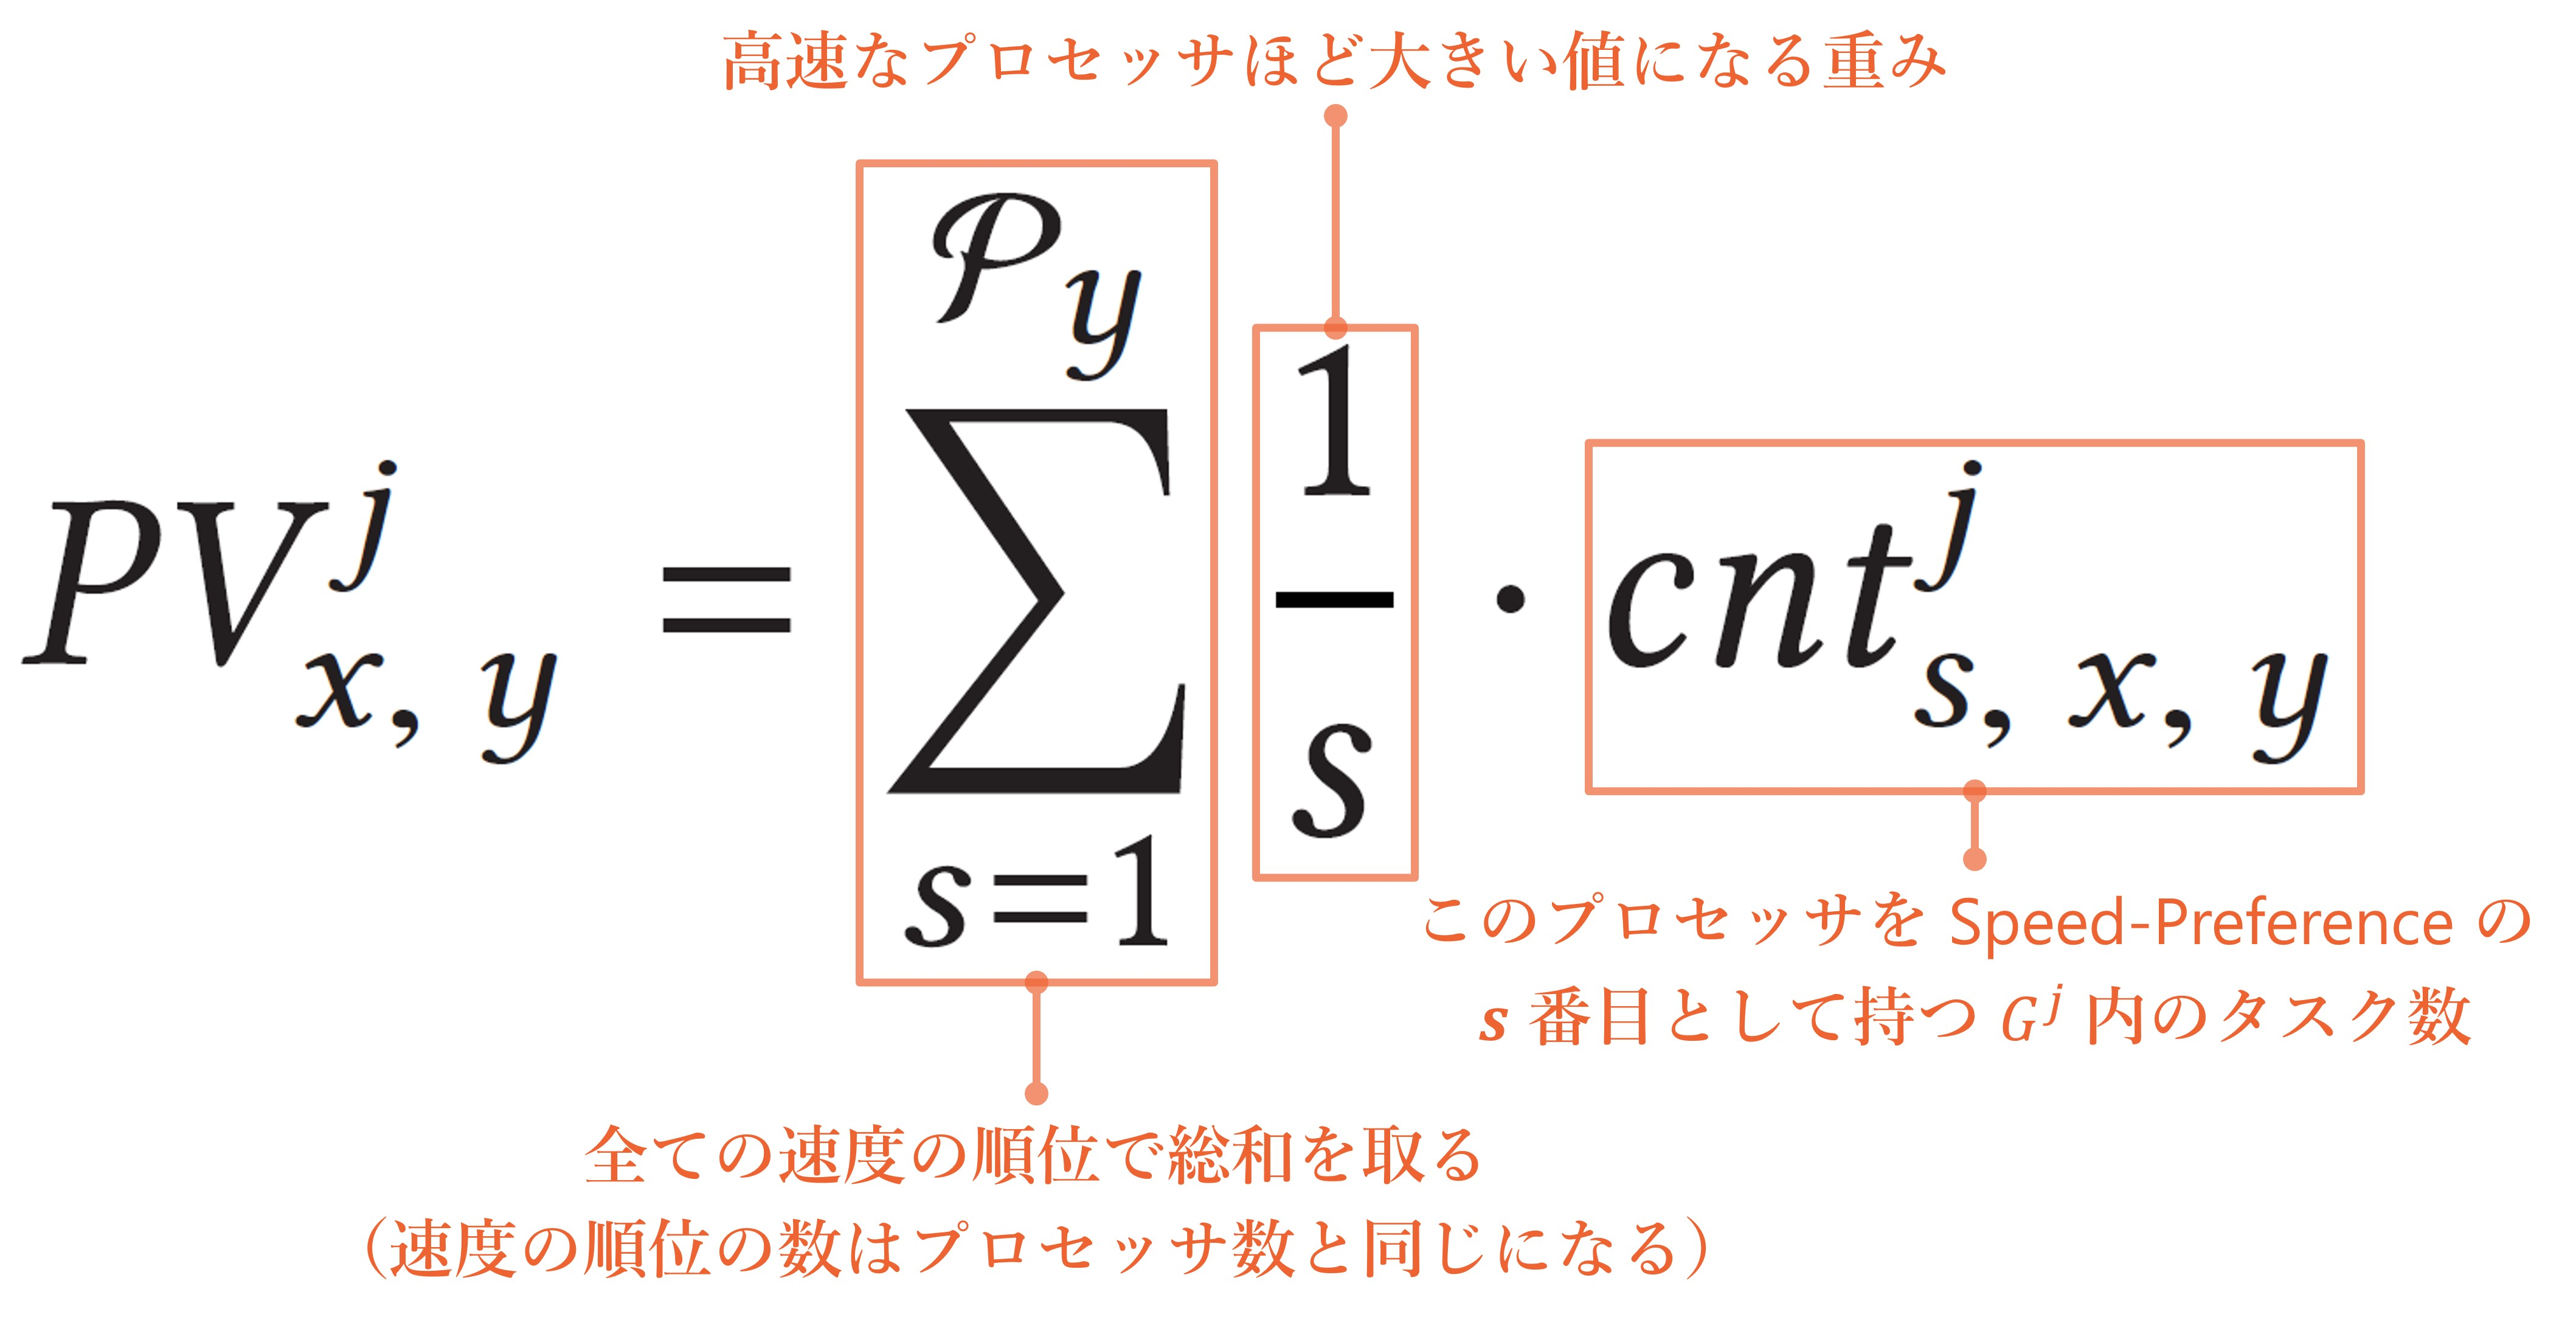
\includegraphics[width=\linewidth]{processor_value}
            }
        \end{figure}
    \end{definition}
\end{frame}

\begin{frame}{クラスタバリュー}
    プロセッサバリューをクラスタバリューに拡張する
    \begin{definition}[$G^j$ に対するクラスタ$\mathcal{K}_y$ のクラスタバリュー]
        \begin{figure}[tb]
            \centering
            \scalebox{0.6}{
                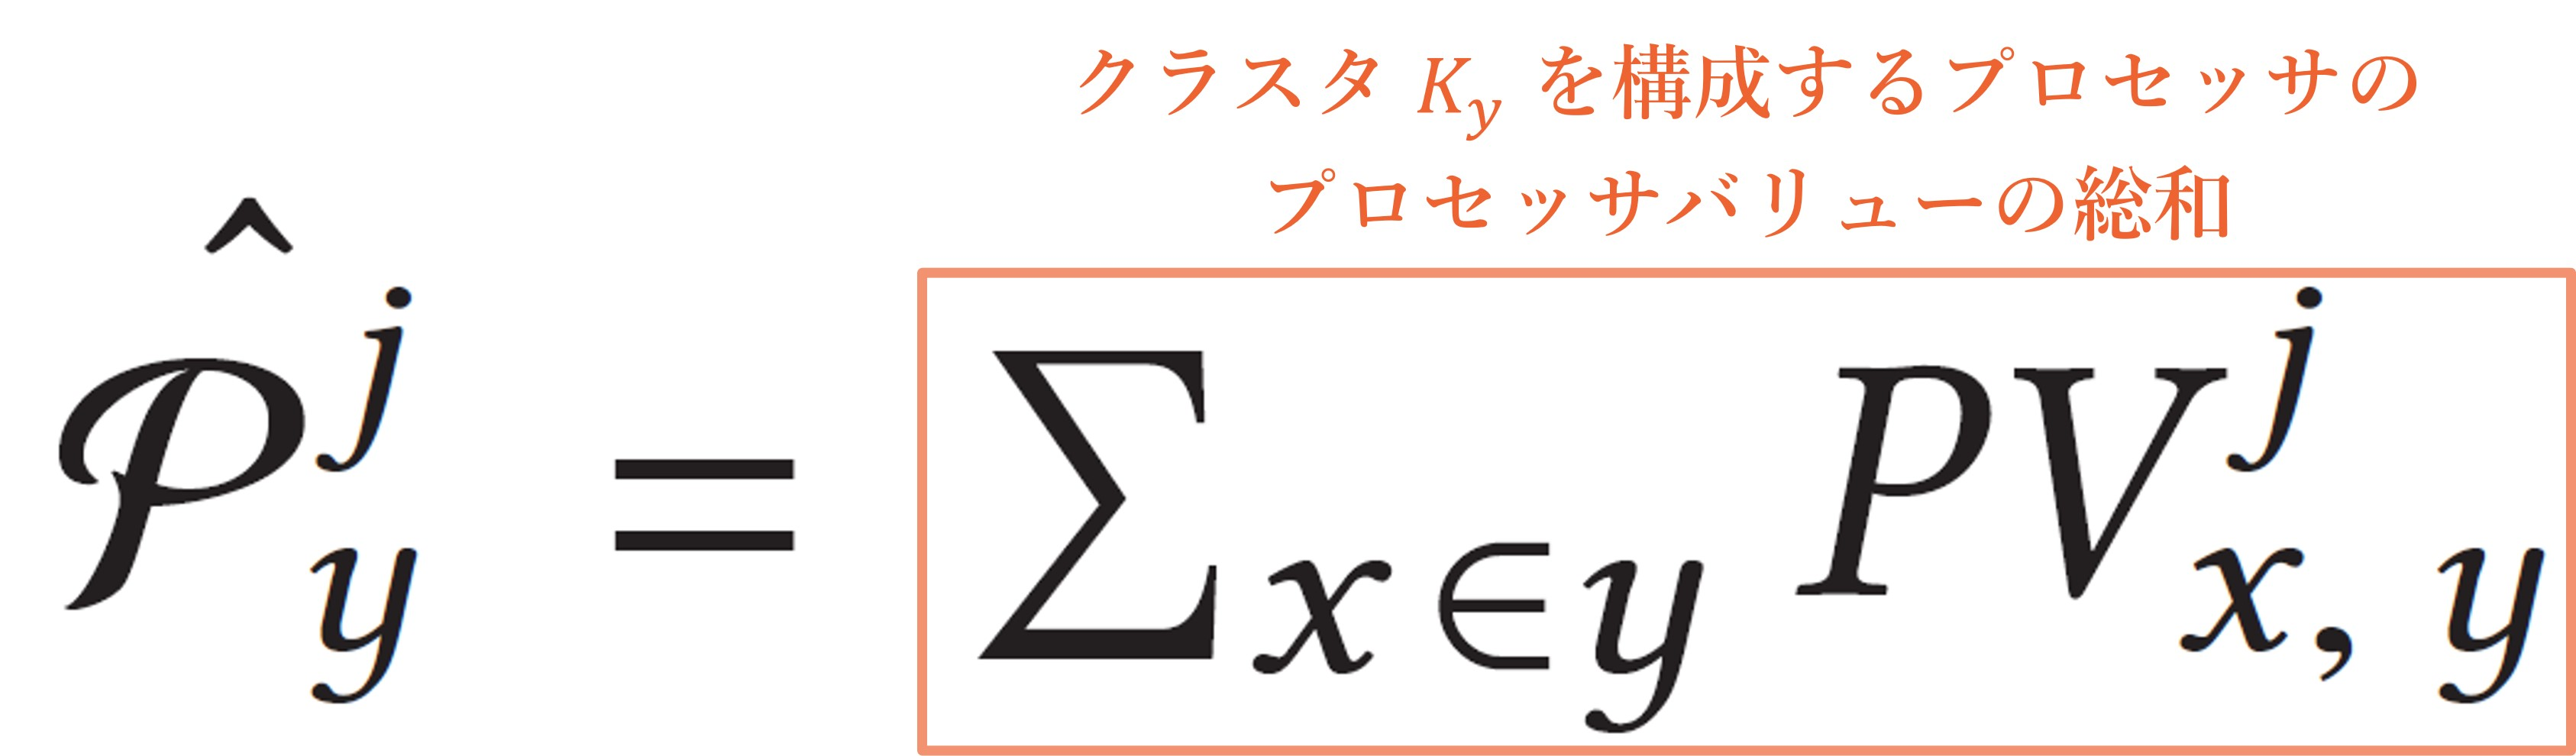
\includegraphics[width=\linewidth]{cluster_value}
            }
        \end{figure}
    \end{definition}
\end{frame}


\subsection{Description of the Algorithm}
\label{ssec: Description of the Algorithm}

\begin{frame}{提案フェデレートスケジューリング全体像}
    \fullimage{fed}
\end{frame}

\begin{frame}{提案フェデレートスケジューリング補足1}
    \fullimage{fed_sup1}
\end{frame}

\begin{frame}{提案フェデレートスケジューリング補足2}
    \fullimage{fed_sup2}
\end{frame}

\begin{frame}{提案フェデレートスケジューリング補足3}
    \fullimage{fed_sup3}
\end{frame}

% !TeX root = main.tex

\section{CAPACITY AUGMENTATION BOUND}
\label{sec: CAPACITY AUGMENTATION BOUND}

\begin{frame}{各アルゴリズムのキャパシティ拡張境界 (証明略)}
    \full{
        \begin{table}[tb]
            \adjustbox{max width=\textwidth, max height=\slideheight}{
                \centering\begin{tabular}{|c|c|} \hline
                                                 & キャパシティ拡張境界                         \\\hline
                    フェデレートスケジューリング & $2$                                  \\\hline
                    グローバルEDF                & $\frac{3 + \sqrt{5}}{2} \cong 2.618$ \\\hline
                    グローバルRMS                & $2 + \sqrt{3} \cong 3.732$           \\\hline
                \end{tabular}
            }
        \end{table}
    }
\end{frame}

\begin{frame}[label=theorem1]{並列タスクのためのキャパシティ拡張境界}
    以下の定理より, コア数 $m$ が十分に大きい場合, フェデレートスケジューリングは最適なキャパシティ拡張境界を示す
    \begin{theorem}[]
        $m$ コア上の並列タスクのための任意のスケジューラのキャパシティ拡張境界の下限は $2-\frac{1}{m}$
        \notes{証明略}
    \end{theorem}
\end{frame}

% !TeX root = main.tex

\section{PRACTICAL CONSIDERATIONS}
\label{sec: Practical Considerations}

\begin{frame}{セクションサマリ}
    \begin{itembox}[l]{\textbf{目的}}
        実用的な観点から, フェデレートスケジューリングの実行効率と有効性を検討する
    \end{itembox}
\end{frame}

% \begin{frame}{}
%     \begin{itemize}
%         \item 前節で示したように, フェデレートスケジューリング, G-EDF, G-RMの容量増大限界はそれぞれ, 2, $2.618$, 3.732である
%         \item 本節では, 実用的な観点から, それらの実行効率と有効性を検討する
%         \item 静的優先度と動的優先度, および, グローバルスケジューリングとパーティショニングスケジューリング, スケジューリングと同期のオーバヘッドによるオーバヘッド, および, 作業保存型と非保存型の4つの次元を考慮する
%     \end{itemize}
% \end{frame}

\begin{frame}{実装のしやすさ}
    \begin{itemize}
        \item 一般に, 動的優先度スケジューラよりも固定優先度スケジューラの方が実装しやすい
        \item フェデレートスケジューリングでは, 高利用率タスクには優先度の割り当てが不要で, 低利用率タスクには固定または動的優先度スケジューラを使用できる
        \item そのため, フェデレートスケジューリングは比較的容易に実装できる
    \end{itemize}
\end{frame}

\begin{frame}{プリエンプション・マイグレーションによるオーバヘッド}
    以下の理由により, フェデレートスケジューリングのオーバヘッドはグローバルスケジューリングより小さいと予想できる
    \begin{itemize}
        \item 各高利用度タスクに最小限の専用コアを割り当てるので, 高利用度タスクのプリエンプションはなく, マイグレーションの回数も最小に抑えられる
        \item シーケンシャル低利用率タスクの場合, プリエンプションとマイグレーションは, より高い優先度を持つ新しいジョブがリリースされたときにのみ発生する
    \end{itemize}
\end{frame}

\begin{frame}{同期やスケジューリングによるオーバヘッド}
    \begin{itemize}
        \item 同期やスケジューリングのオーバヘッドは通常, 各タスクに割り当てられたコア数に対してほぼ線形になる
        \item フェデレートスケジューリングの下では, 最小限のコア数が割り当てられるので, このオーバヘッドは小さい
    \end{itemize}
\end{frame}

\begin{frame}{フェデレートスケジューリングの欠点}
    \begin{itemize}
        \item 多くの実システムでは, 最悪実行時間は悲観的である
        \item フェデレートスケジューリングでは, 最悪実行時間に基づいてタスクに割り当てられたコアは, リソースの過剰供給により, ほとんどの時間アイドル状態になる可能性がある
        \item これに対し, グローバルEDFやグローバルRMは, スレッドマイグレーションにより利用可能なコアを動的に活用できる
    \end{itemize}
\end{frame}

% % !TeX root = main.tex

\section{RELATED WORK}
\label{sec: related_work}

\begin{frame}{既存研究との比較表}
    \full{
        \begin{table}[tb]
            \adjustbox{max width=\textwidth, max height=\slideheight}{
                \centering\begin{tabular}{|c|c|c|c|c|}      \hline
                                                                                                                                                                                & ROS & ROS2 & リアルタイム保証 & 優先度決定 \\\hline
                    \cite{saito2016priority, wei2016rt, saito2018rosch}                                                                                                         & \ch &      &                  &            \\\hline
                    \cite{maruyama2016exploring, gutierrez2018towards}                                                                                                          & \ch & \ch  &                  &            \\\hline
                    \cite{palencia1998schedulability, palencia1999exploiting, davare2007period, schlatow2016response, koren1995skip, abdullah2019worst, becker2016synthesizing} &     &      & \ch              &            \\\hline
                    \cite{casini2019response}                                                                                                                                   & \ch & \ch  & \ch              &            \\\hline
                    本論文                                                                                                                                                      & \ch & \ch  & \ch              & \ch        \\\hline
                \end{tabular}
            }
        \end{table}
    }
\end{frame}

\begin{frame}{ROS のリアルタイム機能の改善}
    以下の研究は ROS のリアルタイム機能の改善に焦点を当てているが, リアルタイムのタイミング制約を保証する分析方法を提供していないか, ROS の第 1 世代にのみ適用されている
    \begin{itemize}
        \item publisherが優先度に基づいてデータを送信できるようにすることで, 優先度に基づくメッセージ送信メカニズムを提案 \cite{saito2016priority}
        \item 2 つのオペレーティングシステムを実行することによって, リアルタイム ROS ノードと非リアルタイム ROS ノードを別々に実行するハイブリッド OS プラットフォームを提案 \cite{wei2016rt}
        \item CPU/GPU 調整メカニズムを備えた ROS のリアルタイム拡張で, ロード可能なカーネルフレームワークである ROSCH-G の提案 \cite{saito2018rosch}
    \end{itemize}
\end{frame}

\begin{frame}{ROS2 のパフォーマンス評価}
    以下の研究は測定ベースのアプローチを使用して ROS2 のパフォーマンスを評価したが, 正式なモデリングや分析は提供していない
    \begin{itemize}
        \item さまざまなベンダー固有の DDS 実装の下でさまざまな QoS 構成を使用して経験的評価を実施 \cite{maruyama2016exploring}
        \item 2 つのノード間の最悪の場合のレイテンシが測定され, PREEMPT-RT パッチが適用された Linux カーネルシステムでデッドラインミスの動作を観察 \cite{gutierrez2018towards}
    \end{itemize}
\end{frame}

\begin{frame}{エンドツーエンドチェーンのレイテンシ分析}
    publisher/subscriber モデルまたは read-execute-write セマンティクスでのエンドツーエンドチェーンレイテンシの分析が行われてきたが, スケジューリングモデルの違いにより, ROS2 に直接適用することはできない
    \setlength{\wideitemsep}{0.8\itemsep}
    {\footnotesize
        \begin{itemize}
            \item マルチコアシステムで優先度の制約があるタスクを分析するためのアプローチ \cite{palencia1998schedulability, palencia1999exploiting}
            \item 最悪の場合の応答時間に基づいて, タスクのエンドツーエンドレイテンシの上界を把握 \cite{davare2007period, schlatow2016response}
            \item 固定優先度スケジューリングの下でチェーンのエンドツーエンドのレイテンシを制限するための分析方法を提示 \cite{koren1995skip, abdullah2019worst, becker2016synthesizing}
            \item チェーンのエンドツーエンドのレイテンシを改善するために, チェーンベースの固定優先度スケジューリングを提案  \cite{choi2020chain}
        \end{itemize}
    }
\end{frame}

\begin{frame}{ROS2 処理チェーンのレイテンシ分析}
    \cite{casini2019response} は ROS2 スケジューラのモデル化とチェーンの応答時間分析の提供に関する唯一の研究だが, リソースを割り当てて, クリティカルチェーンのエンドツーエンドのレイテンシを改善する方法については未検討
    \begin{block}{先行研究 \cite{casini2019response}}
        \setlength{\linewidth}{0.98\columnwidth}
        \setlength{\wideitemsep}{0.8\itemsep}
        {\footnotesize
            \begin{itemize}
                \item エグゼキュータ内のコールバックスケジューリング動作を調査し, リソース予約を使用して, 特定のエグゼキュータのリソースの可用性をモデル化
                \item チェーンのエンドツーエンドのレイテンシは以下の手順で分析される
                      \begin{itemize}
                          {\footnotesize
                          \item エグゼキュータ内の各サブチェーンの応答時間を計算
                          \item CPA~\cite{henia2005system}に基づいてエグゼキュータ全体にまたがるサブチェーンの応答時間を追加
                                }
                      \end{itemize}
            \end{itemize}
        }
    \end{block}
\end{frame}

% !TeX root = main.tex

\section{CONCLUSION}
\label{sec: conclusion}

\begin{frame}{結論}
    \begin{itemize}
        \item ROS 2のための最初の自動レイテンシマネージャであるROS-Llama を提案した
        \item その設計は, ROSエコシステムの要件と制約の慎重な分析によって形作られている
        \item 我々の評価では, ROS-Llamaは実用的で有益であり, デフォルトのCFSベースラインやSCHED\_RRベースラインのいずれよりも負荷の高い状態でより良いレイテンシ制御を達成することが示された
    \end{itemize}
\end{frame}


\lastpage

% \section*{Reference}
% \begin{frame}[allowframebreaks]{Reference}
%     \beamertemplatetextbibitems
%     \bibliographystyle{unsrt}
%     \bibliography{\beamerDir/bibtex/master_reference}
% \end{frame}

\end{document}
